\subsection{Rot-Schwarz-Baum}
Der Rot-Schwarz-Baum stellt eine Erweiterung des bin-ären Suchbaums dar. Er wurde 1972 zum ersten mal von Rudolf Bayer unter dem Namen \glqq symmetric binary B-Tree\grqq{} vorgestellt.

Ein binärer Suchbaum eignet sich zum schnellen Finden von Schlüsselelementen. Dabei werden die Elemente nicht wie in einer Liste sequentiell durchsucht, sondern es wird mit einer bestimmten Logik vorgegangen.
Damit kann eine im Vergleich zur sequentiellen Liste die Laufzeit für verschiedene Operationen verkürzt werden.

Die Anordnung der Elemente wird, wie im Namen bereits enthalten, als Baum vorgenommen. Dabei müssen bestimmte Kriterien für die Anordnung eingehalten werden. Liegt eine bestimmte Anzahl von Elementen vor, die als Binär-Baum angeordnet werden sollen, so wird zunächst ein beliebiges Element ausgewählt und als Wurzel gesetzt. Damit kann es allerdings passieren, dass der Baum später nicht ausgeglichen ist, und alle Äste unterschiedliche Dimensionen aufweisen. Dies würde zu einer unausgewogenen Suche führen. Daher ist es Sinnvoll an dieser Stelle ein Element mit einem Schlüsselwert zu finden, welcher sich relativ in der Mitte der vorkommenden Skala und welcher sich zudem auch bezüglich der Anzahl der Elemente in der Mitte befindet.

Danach werden die nächste Elemente der Reihe nach mit der Wurzel verglichen. Ist das momentan betrachtete Elemente größer als das Wurzel-Element, so wird es an der rechten Seite unter der Wurzel angeordnet. Ist es kleiner als die Wurzel, so kommt es auf die linke Seite. Nun kann das nächste Element mit der Wurzel verglichen werden. Wie im obigen Fall wird es wenn es größer ist der rechten Seite zugeordnet und wenn es kleiner ist der linke Seite. An dieser Stelle kann es jetzt passieren, dass auf der ausgewählten Seite bereits ein Blatt bzw. ein Knoten existiert. Hier muss nun ein weiterer Vergleich stattfinden. Wiederum wird geprüft, ob des momentan ausgewählte Elemente größer oder kleiner ist. Dann wird es unter dieses Element als Blatt angefügt. Somit entsteht ein Baum. Wichtig ist in diesem Verfahren, dass jeder Knoten nur maximal zwei Elemente besitzen kann. 

Die Suche nachher im Baum gestaltet sich ähnlich. Soll ein Element im Baum gesucht werden, so wird ein Vergleich an der Wurzel des Baumes gestartet. Ist der Schlüs\-sel des zu suchenden Elements größer, so wird auf die nächste untere Ebene der rechten Seite gewechselt. Ist der Schlüssel kleiner, dann findet der Wechsel entsprechend auf der linken Seite statt. 

Der größte Vorteil dieser Anordnung besteht wohl in der erheblichen Verkürzung der Laufzeit. 
Als Beispiel soll die Laufzeit beim Suchen dienen.
Während beim sequentiellen Suchen der Maxmimalwert der Laufzeit $O(n)$, mit $n$ als Anzahl der vorhanden Elemente, betragen kann, wird die Laufzeit beim binären Suchbaum auf maximal $O(h)$ verkürzt, wobei $h$ als die Höhe des Baumes betrachtet wird \cite[S.293]{tcormen}

Allerdings kann es auch durch ständiges Löschen und Ein-fügen von Elementen oder aber auch durch eine unvorteilhafte Wahl des Wurzelknotens dazu kommen, dass der Baum aus dem Gleichgewicht gerät. Dies bedeutet, dass eine Seite des Baumes erheblich mehr Knoten besitzt als die andere. Damit würde der Baum in ein Ungleichgewicht fallen. Dadurch wird sich die Suchlaufzeit auf der einen Seite erhöhen und auf der anderen Seite ver\-kürzen. Im Extremfall wären alle Elemente auf einer Seite hintereinander angeordnet und somit wäre die Laufzeit gleich der einer sequentiellen Liste.

Eine solche Fehlanpassung eines Baumes kann mit Hilfe eines Rot-Schwarz-Baumes kompensiert werden. Damit ist es möglich, einen sich ständig ändernden Baum in einem annähernden Gleichgewicht zu halten. 
Der Rot-Schwarz-Baum erweitert einen Binär-Baum mit Hilfe eines Farbattributs für jeden Knoten bzw. für jedes Blatt. Dieses Farbattribut kann in diesem Fall Rot oder Schwarz betragen. Mit Hilfe dieses Attributes können nun bestimmte Regeln aufgestellt werden, welche dann dafür Sorgen das immer ein grundlegenedes Gleichgewicht im Baum herrscht. In Abbildung \ref{fig:rbtree} ist der Aufbau eines Rot-Schwarz-Baumes zu sehen.

\begin{figure}[h]
	\centering
	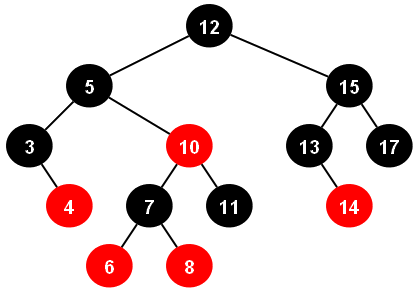
\includegraphics[width=0.45\textwidth]{pictures/redblacktree.png}
%	\caption{RED-BLACK-TREE~\protect\cite{rtoal}}
	\caption{Rot-Schwarz-Baum}
	\label{fig:rbtree}
\end{figure}

 
Nach \cite[S.311]{tcormen} müssen folgende Regeln eingehalten werden, damit ein Baum nach den Prinzipien des Rot-Schwarz-Baumes zustande kommt:

\begin{enumerate}
	\item Jeder Knoten ist entweder rot oder schwarz.
	\item Die Wurzel ist schwarz.
	\item Jedes Blatt (NIL) ist schwarz.
	\item Wenn ein Knoten rot ist, dann sind seine beiden Kinder schwarz.
	\item Für jeden Knoten enthalten alle einfachen Pfade, die an diesem Knoten starten und in einem Blatt des Teilbaumes dieses Knotens enden, die gleiche Anzahl schwarzer Knoten. 
\end{enumerate}


Beim Einfügen bzw. Löschen im binäre Baum werden Verbindungen oder Blätter/Knoten verändert. Damit gerät der Baum immer mehr ins Ungleichgewicht. 
%Mit den Regeln von RED-BLACK wird mit Hilfe von z.B. Rotationen um das den Parent Knoten, immer für das richtige Gleichgewicht gesorgt.
%\newline
\newline
\newline
PROTOTYPE: \newline
WIRD NOCH ERWEITERT UM ERKLÄRUNG DER DEFINITION, EINFÜGEN, SUCHEN, LÖSCHEN
\newline
%\newline
%\newline